\section{Implementation}
In this section, we will describe the implementation of the timed automaton model from the previous section, shown in Figure \ref{fig:automaton}. Our tool of choice is UPPAAL, an integrated solution for modeling, simulation, and verification of timed automata. We will present the implementation details and limitations imposed on the model in the following subsection.  Model variables representing its state will be described along with the most important functions.


\subsection{Model}
The implementation of the timed automaton, shown in Figure \ref{fig:implementation}, includes an additional state called \texttt{grid}, which is not present in the automaton depicted in Figure \ref{fig:automaton}. Global functions of the implementation abstract away the underlying complexity. The  \texttt{grid} state is a consequence of imposing limitations on the environment size defined in the previous section. This allows us to reduce the state space size and perform verification. It is the biggest change made to the original algorithm, defined in Figure \ref{fig:pseudocode}. In that state, it is determined whether a robot has reached the boundary of the grid. If yes, the robot will transition to the state \texttt{turn\_180} and change its direction by 180 degrees as it cannot continue moving forward outside of its environment. If a robot has not reached the boundary of its environment it will transition to the \texttt{if} state where it will transition to further states based on the original rules of the algorithm.

\begin{figure}[H]
\caption{Asynchronous implementation of the Beta algorithm}
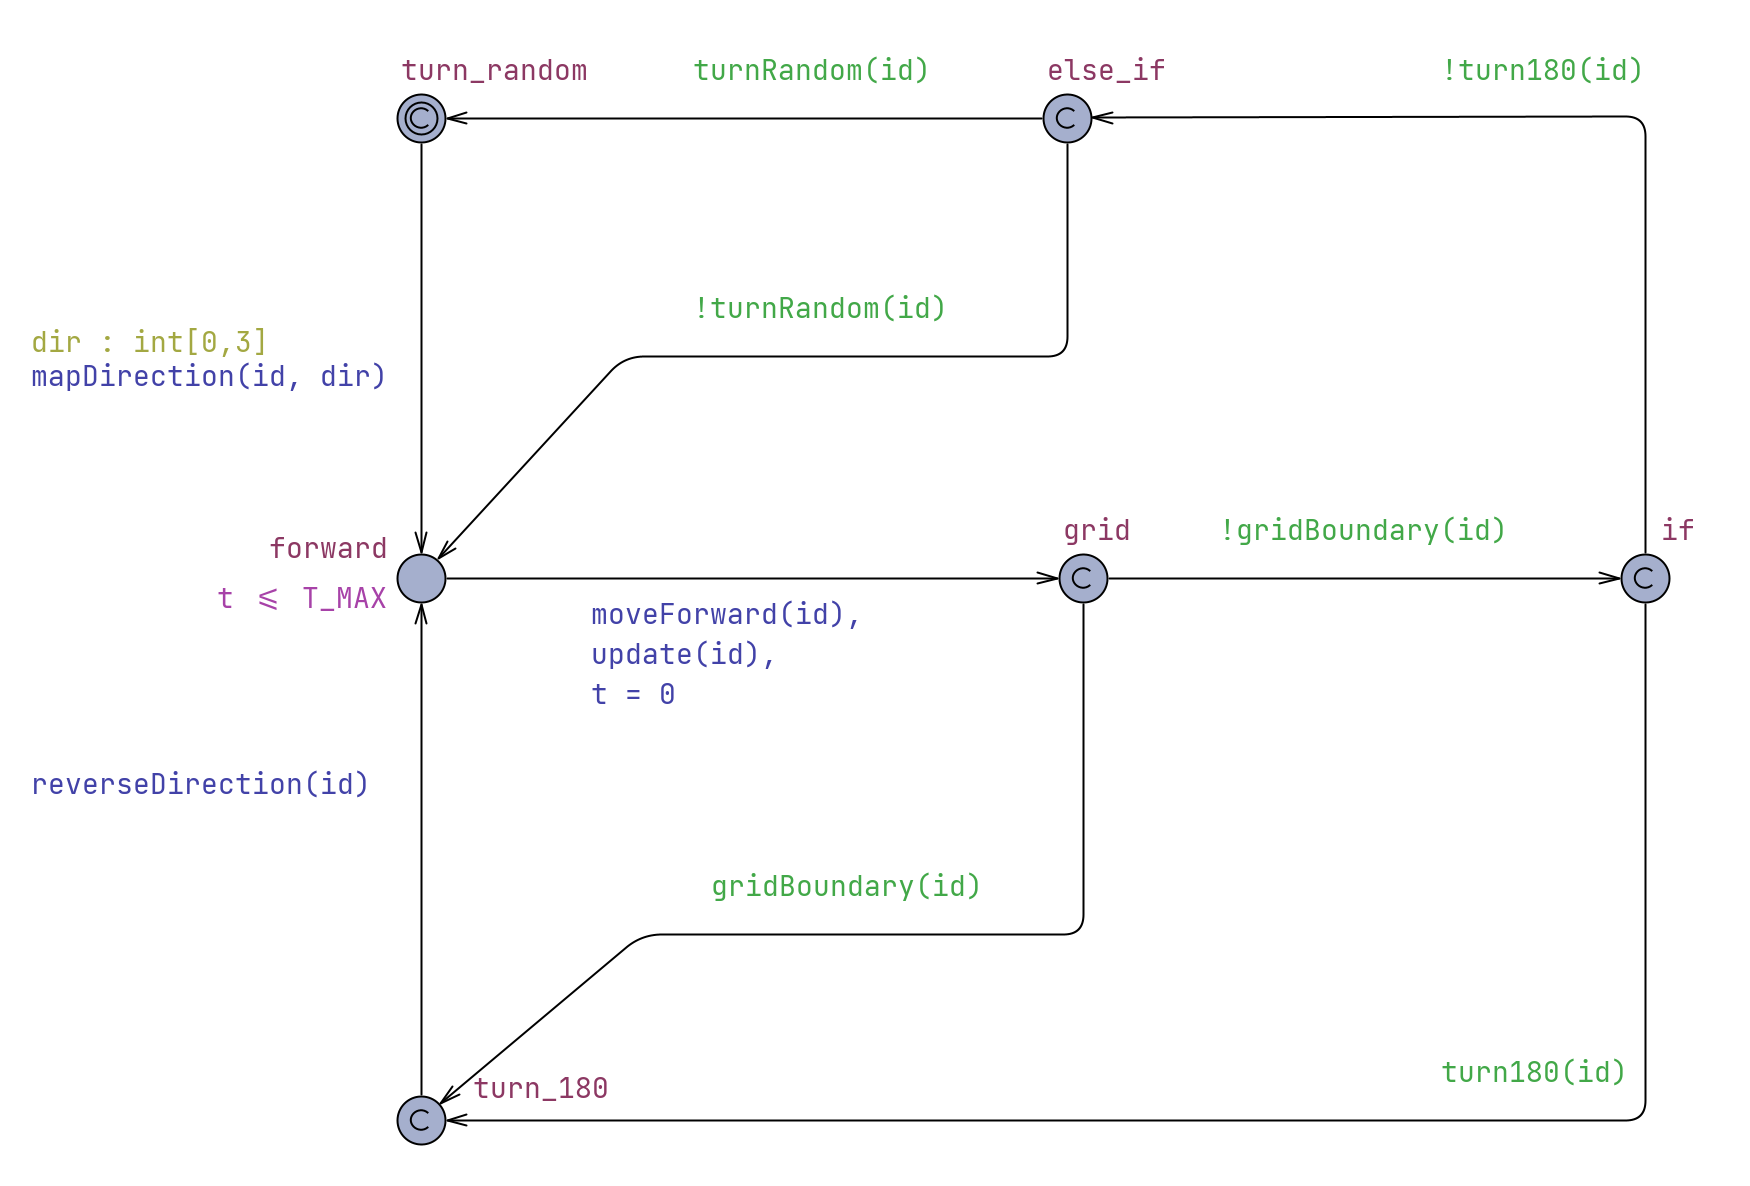
\includegraphics[width=\textwidth]{images/implementation_asynchronous.png}
\label{fig:implementation}
\end{figure}

\noindent
The implementation of the Beta algorithm presented in Figure \ref{fig:implementation} is asynchronous as stated by the author of the algorithm. Robots can move at different pace and time, independent of each other. We also implemented a synchronized version of the Beta algorithm to investigate the influence of the concurrency mode on verification results. The synchronized implementation is presented in Figure \ref{fig:implementation_synchronised}, and its synchronization mechanism in Figure \ref{fig:implementation_synchronised_barrier}. The synchronized version enforces that all robots move at the same time. The synchronization mechanism, which we will call barrier, has a variable \texttt{n} initialized to the number of robots in the swarm. Each time a robot transitions to the \texttt{forward} state it will use a synchronization channel \texttt{done} to notify the barrier. The barrier will decrement its variable \texttt{n} upon receiving a signal from a robot. When the value of \texttt{n} reaches 0, all robots will be blocked in the \texttt{forward} state. The barrier then will send a signal using synchronization channel \texttt{step} and reset the value of the variable \texttt{n} to the number of robots in the swarm. Robots waiting in the \texttt{forward} state will receive this signal from the \texttt{step} channel and transition to \texttt{grid} state at the same time. They will then progress to the \texttt{forward} state in the random order, possibly changing its direction. The order in which they reach the \texttt{forward} state does not influence swarm behavior. A robot decides whether to change direction based on the state of the swarm. The state of the swarm, most importantly robot positions, will not change until the next collective step forward. In other words, the direction of the robot is not a variable that influences the behavior of another robot, unlike its position. 

\begin{figure}[H]
\caption{Synchronised implementation of the Beta algorithm}
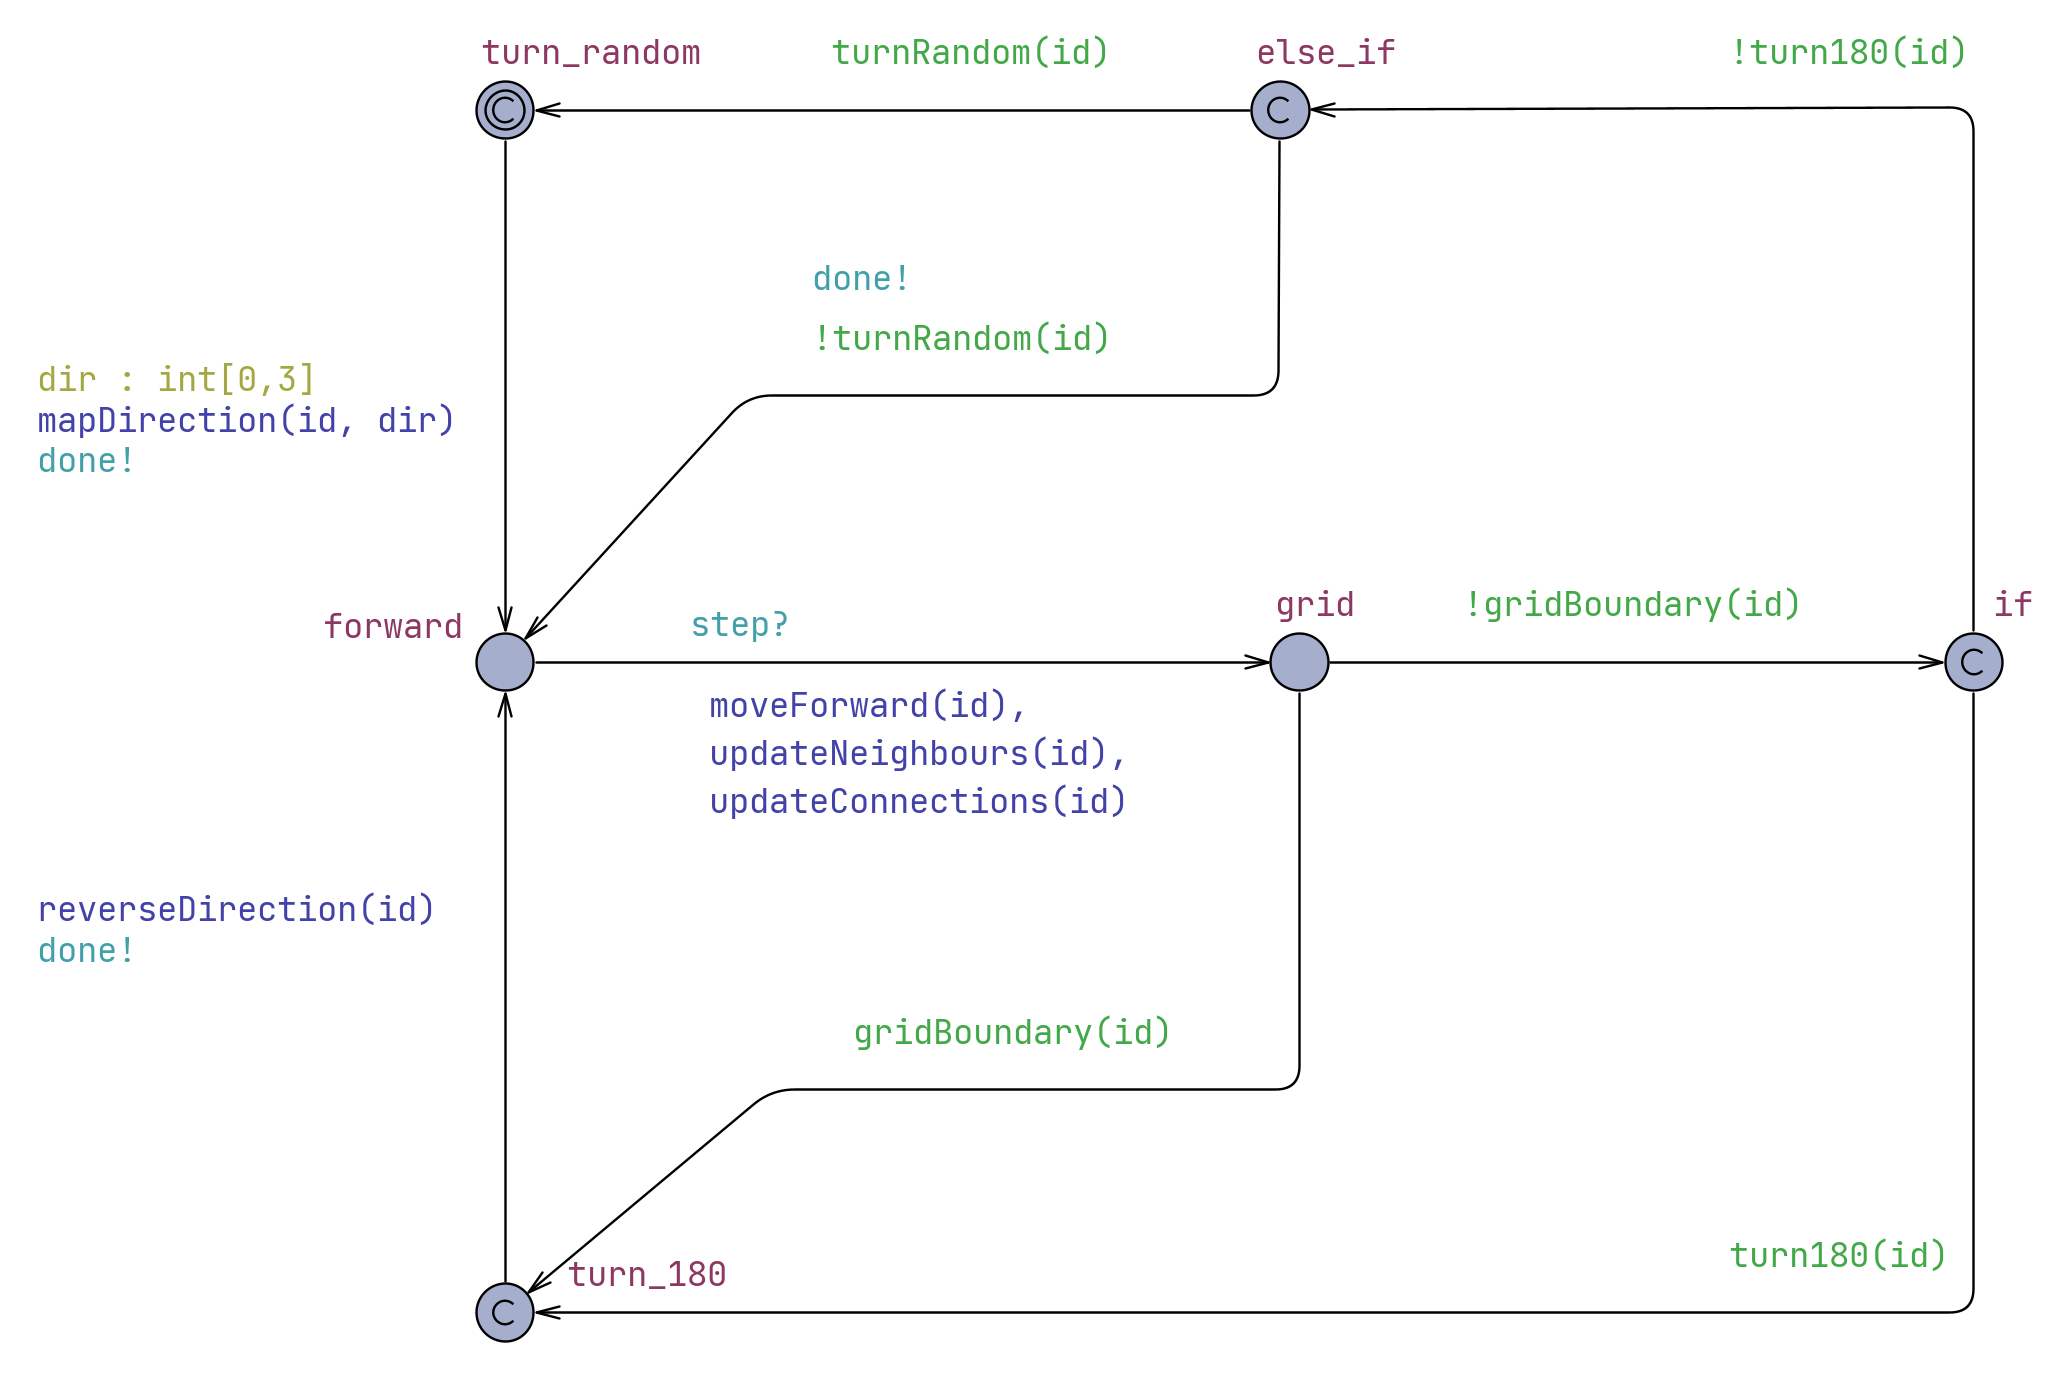
\includegraphics[width=\textwidth]{images/implementation_synchronised.png}
\label{fig:implementation_synchronised}
\end{figure}

\begin{figure}[H]
\caption{Synchronisation mechanism}
\centering
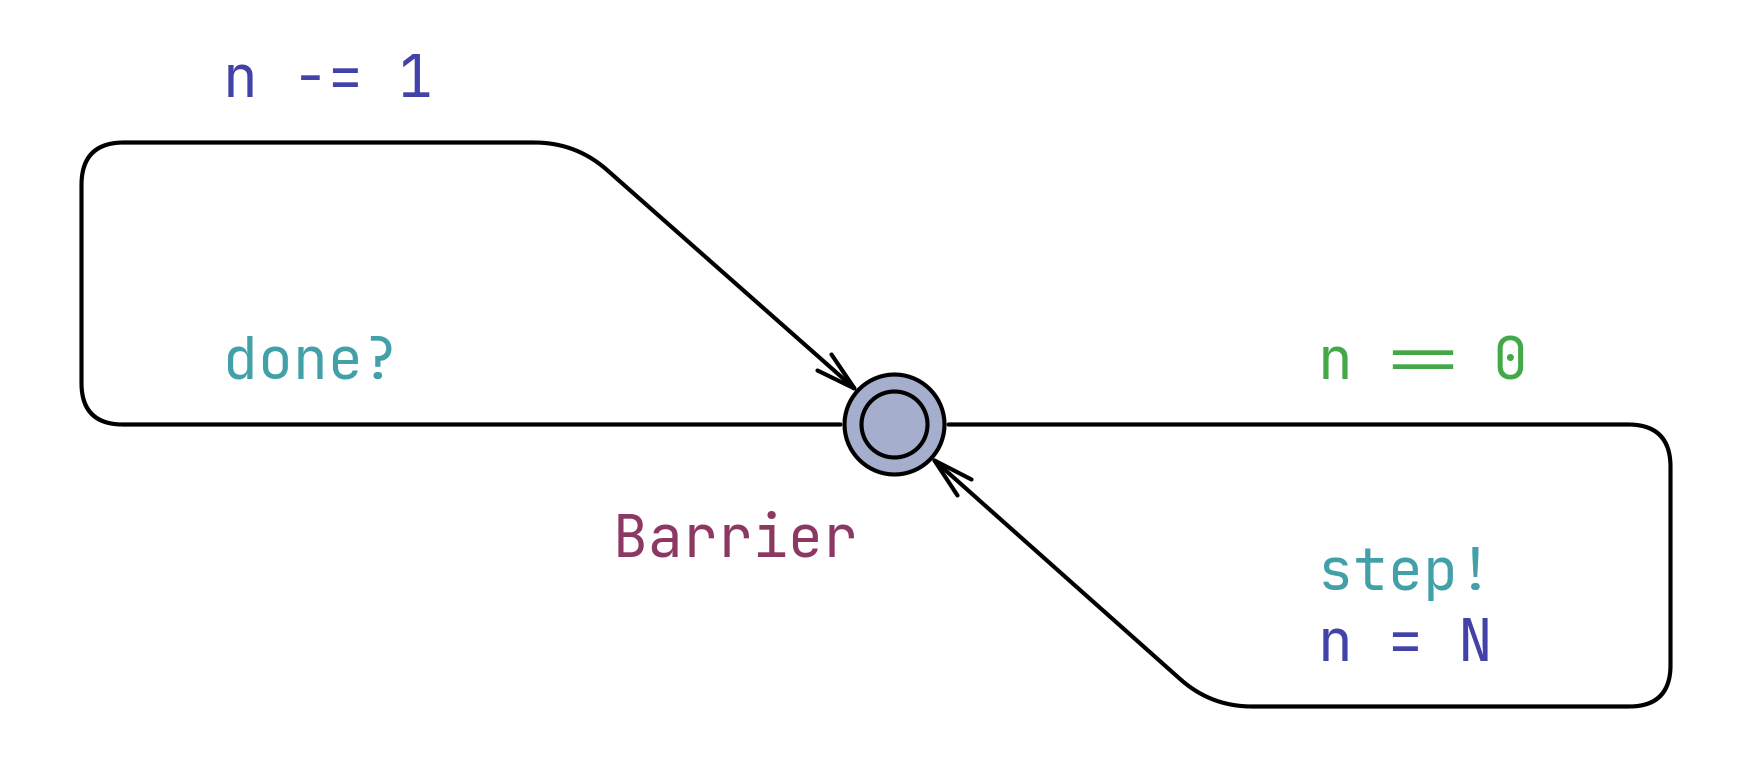
\includegraphics[width=0.5\textwidth]{images/implementation_synchronised_barrier.png}
\label{fig:implementation_synchronised_barrier}
\end{figure}



\subsection{System variables}
Presented below variables fully specify the robot swarm in both asynchronous and synchronised version. Implemented functionality depends on those variables and verified properties are only valid in relation to its values.\\
\texttt{N} - number of robots in a swarm;\\
\texttt{R} - radius of the signal used for connection;\\
\texttt{STEP} - step size of a robot;\\
\texttt{BETA} - beta parameter of the algorithm;\\
\texttt{G} - grid boundary, resulting area of the grid = 2\texttt{G} x 2\texttt{G};\\\\
Asynchronous implementation variables:\\
\texttt{T\_MAX} - time threshold for state invariant;\\
\texttt{C} - global clock for the system;



\subsection{Movement}
Before explaining the functions that control the movement and direction of the robot, we will first introduce the data structures used by these functions.
\\\\
\texttt{x[N]} - list of x-axis coordinates for each robot;\\
\texttt{y[N]} - list of y-axis coordinates for each robot;\\
\texttt{x\_dir[N]} - list of x-axis directions for each robot;\\
\texttt{y\_dir[N]} - list of y-axis directions for each robot;\\
\\
\noindent
Four global functions govern the movement of the robot, namely, \texttt{mapDirection}, \texttt{reverseDirection}, \texttt{moveForward}, \texttt{gridBoundary}. The \texttt{mapDirection} function is triggered upon transition from state \texttt{turn\_random} to state \texttt{forward} and provided with \texttt{id} of the robot and randomly drawn integer \texttt{dir} that will be mapped to one of four directions. The \texttt{reverseDirection} function is triggered upon transition from state \texttt{turn\_180} to state \texttt{forward} and provided with \texttt{id} of the robot whose direction is to be reversed. The \texttt{moveForward} function is triggered upon transition from state \texttt{forward} to state \texttt{grid} and provided with \texttt{id} of the robot that is to be moved forward. The \texttt{gridBoundary} function is used as a transition guard for states \texttt{if} and \texttt{turn\_180}. It takes \texttt{id} of the robot as a parameter. If a robot reaches or crosses the grid boundary it will transition from state \texttt{grid} to state \texttt{turn\_180} and turn 180 degrees to stay within the grid boundary. If a robot has not reached the grid boundary it will transition to the \texttt{if} state and move according to the original specification of the algorithm. The implementation of those functions is shown in Figure \ref{fig:movement_implementation}.


\begin{figure}[H]
\caption{Implementation of functions controlling robot movement}
\begin{lstlisting}[style=C++]
void mapDirection(int id, int dir){
    if (dir == 0){
		// up
        x_dir[id] = 0;
        y_dir[id] = 1;
    }
    if (dir == 1){
		// right
        x_dir[id] = 1;
        y_dir[id] = 0;
    }
    if (dir == 2){
		// down
        x_dir[id] = 0;
        y_dir[id] = -1;
    }
    if (dir == 3){
		// left
        x_dir[id] = -1;
        y_dir[id] = 0;
    }
}


void reverseDirection(int id){
	x_dir[id] *= -1;
	y_dir[id] *= -1;
}


void moveForward(int id){
	x[id] += x_dir[id] * STEP;
	y[id] += y_dir[id] * STEP;
}


bool gridBoundary(int id){
    return abs(x[id]) >= G || abs(y[id]) >= G;
}
\end{lstlisting}
\label{fig:movement_implementation}
\end{figure}
\newpage

\subsection{Connection}
The connection part of the implementation focuses on two key tasks: simulating the physical signal real robots would use to detect their neighbors and providing the functionality and data structures needed for the robots to act on this connection information. A robot will detect its neighbor if the Euclidean distance between them is smaller than signal radius \texttt{R}. Data structures crucial for both of those tasks are listed below. Two-dimensional lists are adjacency matrices where an entry 1 indicates a connection between two robots and 0 indicates the absence of one. \\\\
\texttt{neighbours[N][N]} - is a matrix where each entry is 1 if a robot is currently connected to another robot in the system and 0 if not.;\\
\texttt{last\_neighbours[N][N]} - is a matrix where each entry is 1 if a robot was previously connected to another robot in the system and 0 if not;\\ 
\texttt{lost\_neighbours[N][N]} - is a matrix where each entry is 1 if a robot is currently considered lost as a neighbor of another robot in the system and 0 if not;\\
\texttt{shared\_neighbours[N][N]} - is matrix where each element represents the count of mutual neighbors between each pair of robots in the system;\\
\texttt{shared[N]} - is a list where each element indicates the maximum number of neighbors connected to any one of the lost robots for each robot in the system;\\
\texttt{k[N]} - is a list where each element represents the current number of connections for each robot in the system;\\
\texttt{last\_k[N]} - is a list where each element represents the number of previous connections for each robot in the system;\\
\\
Both of the mentioned tasks are achieved by the \texttt{update} function which controls the state of introduced data structures. Its implementation is presented in Figure \ref{fig:update}. The function updates connection information for only a single robot, the one identified by \texttt{id}. It utilizes the following functions to split the process into logical steps: \texttt{updateNeighbours}, \texttt{lostNeighbours}, \texttt{sharedNeighbours}, \texttt{updateConnections}. Implementation of those steps is presented in Figures \ref{fig:update_3} and \ref{fig:update_1}. It determines the neighbors of the robot based on their positions and signal radius. It checks whether the robot has lost any of the neighbors and if yes it determines how many neighbors are still connected to the lost robot. Finally the function updates current and previous number of connections.

\begin{figure}[H]
\caption{Implementation of \texttt{update} function}
\begin{lstlisting}[style=C++]
void update(int id){
    updateNeighbours(id);
    lostNeighbours(id);
    sharedNeighbours(id);
    updateConnections(id);
}
\end{lstlisting}
\label{fig:update}
\end{figure}


\begin{figure}[H]
\caption{Implementation of functions: \texttt{updateNeighbours}, \texttt{lostNeighbours}, \texttt{updateConnections}}
\begin{lstlisting}[style=C++]
void updateNeighbours(int id){
    // Updates: neighbours, last_neighbours
    int i;
    last_neighbours[id] = neighbours[id];
    for (i = 0; i < N; i++){
        // Check if robots are within signal radius
        if (connected(distance(x[id], y[id], x[i], y[i]), R) 
            && id != i
        ){
            // Connected to i
            neighbours[id][i] = 1;  
        } else {
            // Not connected to i
            neighbours[id][i] = 0;  
        }
    }
}


void lostNeighbours(int id){
    // Updates: lost_neighbours
    int i;
    for (i = 0; i < N; i++){
        // Check if robot lost connection
        if (last_neighbours[id][i] == 1 
            && neighbours[id][i] == 0
        ){
            // Lost connection to i
            lost_neighbours[id][i] = 1;
        } else {
            // Did not loose connection to i
            lost_neighbours[id][i] = 0; 
        }
    }
}


void updateConnections(int id){
    // Updates k, last_k
    int i;
    int n;
    last_k[id] = k[id];
    // Count robot connections
    for (i = 0; i < N; i++){
        if (neighbours[id][i] == 1){
               n++;
        }
    }
    k[id] = n;
}
\end{lstlisting}
\label{fig:update_3}
\end{figure}

\begin{figure}[H]
\caption{Implementation of \texttt{sharedNeighbours} function}
\begin{lstlisting}[style=C++]
void sharedNeighbours(int id){
    // Updates: shared_neighbours, shared
    int i;
    int j; 
    // Clear entries for the robot
    for (i = 0; i < N; i++){
        shared_neighbours[id][i] = 0;
        shared[id] = 0;
    }
    // Check if robot lost any neighbours
    if (noLostNeighbours(id)){
        return;
    }
    // Count neighbours connected to each lost robot 
    for (i = 0; i < N; i++){
        // Check if neighbour 'i' was lost
        if (lost_neighbours[id][i] == 1){
            // Check if robot 'i' is connected to any neighbours
            for (j = 0; j < N; j++){
                if (neighbours[id][j] == 1 
                    && neighbours[j][i] == 1
                ){
                    // Neighbour connected to lost robot 'i'
                    shared_neighbours[id][i] += 1;
                }
            }
        }
    }
    // Find the maximum count of shared neighbours for each lost robot 'i'.
    for (i = 0; i < N; i++){
        if(shared_neighbours[id][i] > shared[id]){
            shared[id] = shared_neighbours[id][i];
        }
    }
}
\end{lstlisting}
\label{fig:update_1}
\end{figure}
\noindent
The function \texttt{updateNeighbours} uses information about robot positions and the radius of the mimicked signal to determine the connectivity of the robot identified by \texttt{id}. It uses \texttt{distance} function to determine the Euclidean distance between two robots and \texttt{connected} function to determine if that distance is smaller or equal to signal radius \texttt{R}. Implementation of functions \texttt{distance} and \texttt{connected} is presented in Figure \ref{fig:update_2}. The function \texttt{lostNeighbours} compares the current and previous state of connectivity of the robot identified by \texttt{id} to determine if the robot has lost any of its connections. The function \texttt{updateConnections} uses data structures updated by the function \texttt{updateNeighbours} to count the number of connections for a robot identified by \texttt{id}. The function \texttt{sharedNeighbours} uses connectivity information of neighbors of the robot identified by \texttt{id} to determine the number of neighbors connected to its lost connections. The algorithm assumption is that a robot can access its neighbors' connectivity information. In other words, the robot is aware of its neighbors' neighbours. The most important information determined by this function is the maximum count of shared neighbors out of all lost connections. This value is compared with \texttt{BETA} parameter to decide whether the robot should turn 180 degrees in an attempt to reconnect with one or more lost robots. The idea behind the implementation of connection was to partition the algorithm into explainable functions and data structures. Even though the functions are global, access to data structures stays at the individual level of the robot, where it is possible. In the case of modeling the physical signal, access to other robot positions was unavoidable.

\begin{figure}[H]
\caption{Implementation of functions: \texttt{distance}, \texttt{connected}}
\begin{lstlisting}[style=C++]
double distance(int x1, int y1, int x2, int y2){
    return sqrt(pow(abs(x1-x2),2) + pow(abs(y1-y2),2));
}


bool connected(double distance, double threshold){
    return distance <= threshold;
}
\end{lstlisting}
\label{fig:update_2}
\end{figure}